\section{Application}
The box-transportation problem is significant in both the theoretical and practical domain. From a theoretical point of view, it is a relatively simple problem with clear boundaries. Although there are multiple versions of this problem, the basic idea is intuitively easy to understand. Because of its simplicity, it is not hard to extend it to more complicated, real-life situations. It is also a good task to observe the effects of different learning algorithms since, in the more simple, stripped down versions of this task, there are not a lot of parameters that influence the outcome. Finally, it is an interesting way of studying cooperation between multiple autonomous agents.

 Although we use a simulation in this paper, the task has successfully been completed by physical robots. For example, in \cite{mataric2002} a team of two Pioneer 2 mobile robots was used to physically push a box to a goal area while a third robot served as an observer. In \cite{kube1996} they took a different approach, where they used a swarm of smaller custom robots to collectively move a box to a designated spot (as can be seen in figure \ref{1}).
\begin{wrapfigure}[15]{r}{0.5\textwidth}
	\centering
	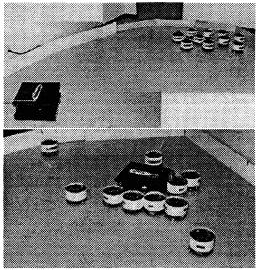
\includegraphics{images/swarmPushing.png}
	\caption{Robots from \cite{kube1996} locating a lit box.}
	\label{1}
\end{wrapfigure}
It is not hard to come up with practical applications for these kind of systems. In the future, they might for example be useful in construction, or to clear the rubble after a building has collapsed.\\
